\lstset{numbers=none}

\section{Spécification du protocole de communication} % (fold)

Cette section décrit la partie technique du projet.
Elle vous permettra de réaliser la partie communication de votre joueur.

Lors d'une partie, plusieurs programmes sont exécutés : le programme des joueurs et un programme (appelé serveur) qui coordonne toutes les actions.
Au début d'une partie, le serveur envoie toutes les informations nécessaires pour le bon déroulement d'une partie (cf \ref{initial}).
Ensuite, à chaque début de tour et pour chaque joueur, le serveur envoie les données courantes et attend en réponse les actions à réaliser (cf \ref{input} et \ref{output}).
Pour finir, une fois qu'une partie se termine pour un joueur (en cas de défaite ou de victoire), le serveur envoie des dernières données au joueur (cf \ref{final}).

\subsection{Serveur de jeu} % (fold)

Le serveur de jeu est un programme qui vous est fourni.
Il permet de lancer des parties, coordonner les joueurs, vérifier les mouvements, vous fournir les données courantes de la partie, etc.
C'est également lui qui gère les entités non jouables (humains, berzerks).
La section \ref{outils} décrit comment utiliser ce serveur de jeu.

La communication avec le serveur de jeu se base sur le protocole TCP\footnote{http://en.wikipedia.org/wiki/Transmission\_Control\_Protocol}.
C'est la forme la plus commune d'échanger des données sur le réseau.
Lorsqu'il s'agit de communiquer en TCP, chaque langage propose son API\footnote{généralement appelé Socket}.
De nombreux exemples peuvent être trouvés sur internet\footnote{par exemple: http://pleac.sourceforge.net}.
Lorsque vous lancez votre programme, vous connaissez l'adresse du serveur et vous êtes donc capable de communiquer avec lui.

\begin{figure}[htbp]
    \centering
    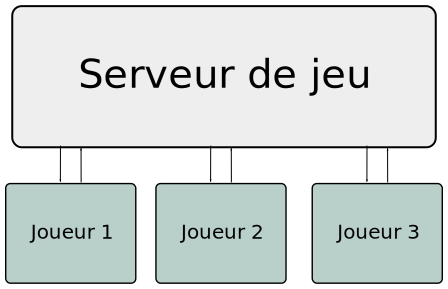
\includegraphics[width=0.5\textwidth]{pics/archi_client_serveur}
    \caption{Architecture Client-Serveur du jeu}
    \label{archi}
\end{figure}

La Figure~\ref{archi} représente le comportement global des programmes lors d'une partie.
Le serveur est le point central et est le seul à avoir la connaissance totale de toutes les données.


% subsection Serveur de jeu (end)

\subsection{Échanges initiaux} % (fold)
\label{initial}
Avant que le jeu ne commence réellement, le serveur et un joueur échangent quelques messages.
Il faut noter que dans tous les échanges suivants, un message commençant par "$<$" sera envoyé du serveur vers le joueur et un message commençant par "$>$" sera envoyé du joueur vers le serveur.
Les mots affichés en bleu sont des mots-clés du protocole.

De plus, les paramètres envoyés en début de partie seront envoyés de la manière suivante: \lstinline!name value!.

\subsubsection{Identification} % (fold)
\label{identification}
Le joueur s'identifie auprès du serveur.

\begin{lstlisting}
>  nick  pseudo
<  nick  pseudo    noPlayer 
\end{lstlisting}

Le pseudo retourné par le serveur n'est pas forcément identique à celui envoyé initialement.
En effet, si deux joueurs donnent le même pseudo, il faut les différencier.
Également, le serveur retourne le numéro d'équipe du joueur.

% subsubsection Identification (end)

\subsubsection{Paramètres de la partie} % (fold)

Les paramètres sont ensuite données de la manière suivante :

\begin{lstlisting}
<  init
<  attack_radius     value
<  berzerk_delay     value
<  berzerk_radius    value
<  bullet_amount     value
<  cols              value
<  contagion_amount  value
<  contagion_radius  value
<  move_len          value
<  nb_team           value
<  rows              value
<  shot_radius       value
<  shot_success      value
<  timing_limit      value
<  turn_max          value
<  view_radius       value
<  end
\end{lstlisting}

Attention, les paramètres ne sont pas forcément donnés dans cet ordre.
De plus, les paramètres peuvent être des flottants ou des entiers.


% subsubsection Paramètres de la partie (end)

% subsection Données initiales et de début de tour (end)

\subsection{Tour par tour : Input} % (fold)
\label{input}

\subsubsection{Données générales} % (fold)
À chaque tour, le serveur actualise les informations du joueur.
Cela commence de la manière suivante :

\begin{lstlisting}
<  turn  turnNo
\end{lstlisting}
\begin{center}
OU
\end{center}
\begin{lstlisting}
<  end
\end{lstlisting}

Dans le deuxième cas, cela annonce que le joueur est vaincu ou bien que la partie est terminée.
Le joueur reçoit alors les données finales (cf \ref{final}).
Si le joueur est toujours en jeu, il reçoit alors les informations courantes de la partie :

\begin{lstlisting}
< players nbPlayersLeft
< scores p1Score ... pnScore
\end{lstlisting}

\subsubsection{Données courantes de la carte} % (fold)

Ensuite, le serveur envoie toutes les données que le joueur peut percevoir.
Ces informations sont formatées de la manière suivante :

\lstset{numbers=left}
\begin{lstlisting}
<  water      row  col
<  entity     row  col     type  team
<  shot       id
<  contagion  id   id_new  row   col   nb_bullets
<  zombie     id   row     col
<  dead       id
\end{lstlisting}
\lstset{numbers=none}


La ligne \lstinline!1! correspond à une case de type \water{} nouvellement découverte à la position \lstinline!(row, col)!.

La ligne \lstinline!2! correspond à la présence d'une entité (d'une autre équipe) à la position \lstinline!(row, col)!.
Cette entité peut être de plusieurs types : \human{}, \cop{}, \zombie{} ou \berzerk{}.
L'entité peut être rattaché à son équipe (par convention, les entités non jouables appartiennent à l'équipe \lstinline!0!).
Un joueur connait son équipe lors de la phase d'identification (cf \ref{identification}).

La ligne \lstinline!3! correspond à une tentative réussie de tir de la part d'un zombie policier \emph{du joueur}.
Le zombie policier est identifié grâce à son \lstinline!id!.

La ligne \lstinline!4! signifie qu'un zombie \emph{du joueur} (identifié par \lstinline!id!) a réussi à contaminer un humain.
Le nouveau zombie (identifié par \lstinline!id_new!) si situe à la position \lstinline!(row, col)!.
Si le nouveau zombie était un humain, \lstinline!nb_bullets! vaudra 0, sinon il vaudra le nombre de balles restantes du policier.

La ligne \lstinline!5! indique que le zombie \emph{du joueur} d'identifiant \lstinline!id! s'est déplacé à la position \lstinline!(row, col)!.
Cette commande est également utilisée lors du premier tour pour placer le ou les zombies initiaux.

La ligne \lstinline!6! désigne un zombie \emph{du joueur} qui est mort au tour précédent.

Lorsque toutes les nouvelles informations sont communiquées au joueur, le serveur notifie le joueur qu'il attend ses instructions :
\begin{lstlisting}
<  end
\end{lstlisting}


% subsubsection Données générales (end)

% subsection Données de chaques tours (end)

\subsection{Tour par tour : Output} % (fold)
\label{output}
Lorsqu'un joueur a reçu toutes les données courantes du tour, il doit prendre des décisions, bouger ou non ses unités.
Pour cela, il peut envoyer au serveur des ordres de mouvement :
\begin{lstlisting}
>  move  id  dir
\end{lstlisting}
Cet ordre consiste de déplacer le zombie \lstinline!id! dans la direction \lstinline!dir!.
La direction peut être égale à \north{}\lstinline!=N!, \east{}\lstinline!=E!, \south{}\lstinline!=S!, \west{}\lstinline!=W!.

Une fois que le joueur a envoyé l'ensemble de ses ordres, il notifie le serveur :
\begin{lstlisting}
>  end
\end{lstlisting}


% subsection Données relatives aux décisions du joueur (end)

\subsection{Données finales} % (fold)
\label{final}

Une fois que le joueur est déclaré vainqueur ou perdant, il reçoit les informations suivantes :

\begin{lstlisting}
<  final   type     turnNo
<  scores  p1Score  ...     pnScore
\end{lstlisting}

Un joueur peut savoir s'il a gagné grâce à \lstinline!type!, qui vaut \lstinline!1! si le joueur est vainqueur, \lstinline!0! sinon.
Pour finir, il peut savoir après combien de tour s'est terminée la partie, grâce à \lstinline!turnNo!.
Les scores finaux sont ensuite transmis au joueur.


% subsection Données finales (end)

% section Spécification (end)
